\clearpage
\section{Resultados de las pruebas}

Las pruebas de aceptación de los tres sprints se volvieron a ejecutar el 25 de noviembre de 2026 sobre la versión final
del sistema (rama \texttt{develop}, commit \texttt{ac93ec4}) funcionando en el computador del equipo con Docker Compose:
interfaz web, API Gateway, los tres microservicios, RabbitMQ, SQL Server (una base por servicio) y Ollama. Cada rol
(Operador, dos Docentes revisores y Administrador) trabajó en una ventana de navegador separada, con su propia sesión.
Las capturas se tomaron directamente de la aplicación en ese momento y están en la carpeta \texttt{capturas}, con el
mismo orden y número de esta sección.

Como en el Sprint 2, las pruebas que no tienen pantalla se respaldan con la salida de la consola (RabbitMQ y SQL Server)
o con las pruebas automáticas del proyecto, que se ejecutan en la integración continua. Las pruebas del Sprint 1 y del
Sprint 2 cuya pantalla cambió por las correcciones de la sección~\ref{sec:correcciones} se ejecutaron sobre la pantalla
actual; cuando una prueba ya no aplica se indica la corrección que la reemplazó.

\textbf{Datos de prueba utilizados:} los certificados SIHA de la carpeta \texttt{documentos-prueba/certificados-pruebas}
(V02 a V07 válidos; E05, E06, E10, E18, E19 y E20 con errores), los sílabos oficiales de la UTA cargados en el
Microservicio A y los sílabos de la ESPOCH para la movilidad externa. Docentes revisores: Ing.~Carlos Paredes e Ing.~María Vaca.

% =====================================================================
\subsection{Sprint 1: base del sistema (HU-01 a HU-06)}

\subsubsection{HU-01 -- Gestionar cuentas y roles}

\prueba{PA-01.1: Lista de cuentas con su rol y estado}
{El administrador abre Usuarios y roles.}
{pa01-1-cuentas.png}{Cuentas registradas con su rol y estado (HU-01)}
{Se listan las cuentas institucionales con su rol (Administrador, Docente, Operador), su estado y su último acceso.
Cada fila ofrece Editar, Restablecer contraseña, Desactivar y Dar de baja.}{0.95}

\prueba{PA-01.2: Crear una cuenta con datos que no coinciden}
{El administrador intenta crear una cuenta escribiendo dos contraseñas distintas.}
{pa01-2-validacion.png}{Validación al crear una cuenta (HU-01)}
{El campo Confirmar contraseña se marca en rojo con el mensaje ``Las contraseñas no coinciden.'' y la cuenta no se crea.
El rol viene marcado como Operador por defecto, el de menos permisos.}{0.95}

\prueba{PA-01.3: Un rol sin permiso entra a Usuarios y roles}
{El operador escribe a mano la dirección de Usuarios y roles.}
{pa01-3-acceso-denegado.png}{Aviso de acceso para un rol sin permiso (HU-01)}
{El sistema muestra ``No tiene acceso a esta sección'' con el rol autorizado y el rol con el que entró, en lenguaje
sencillo y con los botones Ir al inicio y Cambiar de cuenta.}{0.95}

\subsubsection{HU-02 -- Configurar reglas y umbrales}

\prueba{PA-02.1: Reglas vigentes y catálogo normativo}
{El administrador abre Configurar mínimo (80~\%).}
{pa02-1-reglas.png}{Reglas y umbrales vigentes (HU-02)}
{Se muestra el contenido mínimo (80~\%) con su versión y el catálogo normativo. La regla RN-01 ya indica que los
créditos son obligatorios y que los contenidos solo generan una recomendación.}{0.80}

\prueba{PA-02.2: Intentar bajar el mínimo de 80~\%}
{El administrador escribe 70 en Contenido mínimo y guarda.}
{pa02-2-minimo.png}{El mínimo no se puede bajar de 80~\% (HU-02)}
{Aparece ``El contenido mínimo no puede ser menor que 80~\%: lo fija el reglamento de homologación de la UTA. Puede
exigir más, pero no menos.'' y no se guarda nada.}{0.95}

\subsubsection{HU-03 -- Gestionar carreras, mallas y asignaturas}

\prueba{PA-03.1: Carreras y versiones de malla}
{El administrador abre Carreras y mallas.}
{pa03-1-mallas.png}{Carreras de la FISEI y sus mallas (HU-03)}
{Se listan las carreras de la FISEI con sus versiones de malla, que son las que usa el agente para comparar.}{0.95}

\prueba{PA-03.2: Asignaturas con créditos, horas y unidades}
{El administrador abre Asignaturas y contenidos.}
{pa03-2-asignaturas.png}{Asignaturas y unidades temáticas (HU-03)}
{Cada asignatura muestra su nivel, créditos, horas y unidades temáticas cargadas desde los sílabos oficiales.}{0.95}

\subsubsection{HU-04 -- Entrada única por el API Gateway}

\prueba{PA-04.1: Petición sin iniciar sesión}
{Se pide la lista de usuarios al Gateway sin enviar el JWT.}
{pa04-1-401.png}{El Gateway rechaza la petición sin JWT (HU-04)}
{El Gateway responde \textbf{401 Unauthorized} y la petición no llega al Microservicio A.}{0.95}

\prueba{PA-04.2: Un docente pide un recurso de administrador}
{Con la sesión del docente Carlos Paredes se pide la lista de usuarios.}
{pa04-2-403.png}{El Gateway rechaza un rol sin permiso (HU-04)}
{El Gateway valida el JWT pero responde \textbf{403 Forbidden}, porque la gestión de cuentas es solo del Administrador.}{0.95}

\subsubsection{HU-05 -- Registrar solicitudes con su documento}

\prueba{PA-05.1: Archivo que no es el certificado}
{El operador sube un plan analítico suelto (E19) en lugar del certificado.}
{pa05-1-rechazo.png}{Rechazo de un documento que no es el certificado SIHA (HU-05)}
{Aparece ``Este PDF no es el certificado SIHA'' con el motivo, y el botón de registrar queda deshabilitado.}{0.95}

\prueba{PA-05.2: Registro de un certificado válido}
{El operador sube el certificado V05 y lo registra.}
{pa05-2-registro.png}{Solicitud registrada y enviada (HU-05)}
{Se crea el expediente con su código, se muestran el estudiante, el cambio de carrera, las materias pedidas y los
docentes revisores, y se indica que el agente ya está analizando.}{0.95}

\subsubsection{HU-06 -- Avisar a los otros servicios}

\prueba{PA-06.1: Publicación del evento en RabbitMQ}
{Después de registrar, se consultan las colas de RabbitMQ y el registro del Microservicio C.}
{pa06-1-rabbitmq.png}{Cola, intercambio del evento y procesamiento en MS C (HU-06)}
{Existe el intercambio \texttt{SolicitudCreadaEvent} y la cola \texttt{solicitud-creada-ms-c} con un consumidor y cero
mensajes pendientes. El registro de MS C muestra ``SolicitudCreadaEvent procesado'' para las solicitudes registradas.}{1.0}

\begin{table}[H]\centering\small
\begin{tabularx}{\textwidth}{|l|X|X|l|}\hline
\rowcolor{grisTarjeta}\textbf{N.º} & \textbf{Prueba} & \textbf{Resultado obtenido} & \textbf{Estado}\\\hline
PA-01.1 & Lista de cuentas & Cuentas con rol, estado y acciones & Cumple\\\hline
PA-01.2 & Datos que no coinciden & ``Las contraseñas no coinciden''; no se crea & Cumple\\\hline
PA-01.3 & Rol sin permiso & ``No tiene acceso a esta sección'' & Cumple\\\hline
PA-02.1 & Reglas vigentes & Mínimo 80~\% y catálogo RN & Cumple\\\hline
PA-02.2 & Bajar de 80~\% & Rechazado con mensaje claro & Cumple\\\hline
PA-03.1 & Carreras y mallas & Listado de carreras y versiones & Cumple\\\hline
PA-03.2 & Asignaturas & Créditos, horas y unidades & Cumple\\\hline
PA-04.1 & Sin JWT & 401 en el Gateway & Cumple\\\hline
PA-04.2 & Rol sin permiso & 403 en el Gateway & Cumple\\\hline
PA-05.1 & Documento equivocado & Rechazado; botón deshabilitado & Cumple\\\hline
PA-05.2 & Certificado válido & Expediente creado y enviado & Cumple\\\hline
PA-06.1 & Evento en RabbitMQ & Evento publicado y procesado & Cumple\\\hline
\end{tabularx}
\caption{Resultados de las pruebas del Sprint 1}
\end{table}

% =====================================================================
\clearpage
\subsection{Sprint 2: análisis de la solicitud (HU-07 a HU-11)}

Se repiten las 23 pruebas del documento del Sprint 2 con su mismo número. Desde la corrección C-01 el documento de
entrada es el certificado SIHA (ya no el plan analítico suelto), por eso las pruebas de lectura se ejecutan con él.

\subsubsection{HU-07 -- Leer el documento y confirmar los datos dudosos}

\prueba{PA-07.1: Lectura de un PDF con texto}
{El operador sube el certificado V05 (Industrial a Software).}
{pa07-1-datos-leidos.png}{Datos leídos del certificado (HU-07)}
{El sistema muestra el estudiante, el trámite, el certificado, los docentes revisores, las materias pedidas y el
historial académico completo con nivel, período, nota y estado.}{0.70}

\prueba{PA-07.2: Aviso de solicitud repetida}
{El operador vuelve a registrar el certificado V02, que ya estaba registrado.}
{pa07-2-repetido.png}{Aviso de certificado ya registrado (HU-07)}
{Junto al botón aparece ``El certificado SIHA-2026-0202 ya fue registrado en el expediente…'' con el enlace Ver la
solicitud registrada; no se crea una segunda solicitud. Que un mismo aviso de RabbitMQ no cree dos análisis lo
comprueba la prueba automática \texttt{Ignora\_evento\_duplicado\_sin\_crear\_otro\_registro}.}{0.95}

\prueba{PA-07.3: Lectura con datos que faltan}
{El operador sube el certificado E20, que tiene la cédula vacía y una materia sin período.}
{pa07-3-campos-vacios.png}{Certificado con campos sin llenar (HU-07)}
{La revisión muestra ``El certificado tiene campos sin llenar'', con la lista de verificación por sección y el botón
de registrar deshabilitado. El análisis no empieza.}{0.80}

\prueba{PA-07.4: Confirmar con datos vacíos}
{En el registro manual el operador pulsa Revisar los datos sin llenar el formulario.}
{pa07-4-manual-vacio.png}{Registro manual con datos vacíos (HU-07)}
{Se muestra la lista de lo que falta por sección y no se guarda nada.}{0.55}

\prueba{PA-07.5: PDF escaneado}
{El operador sube un PDF escaneado (E18).}
{pa07-5-escaneado.png}{PDF escaneado rechazado (HU-07)}
{Aparece ``Este PDF no es el certificado SIHA'' y se explica que el certificado debe generarse digitalmente; el
sistema no inventa datos.}{0.95}

\subsubsection{HU-08 -- Calcular con las reglas y umbrales aprobados}

\prueba{PA-08.1: Reglas en el resultado}
{Se abre el análisis de una solicitud y se revisa la sección Reglas de homologación.}
{pa08-1-reglas-en-resultado.png}{Reglas aplicadas en el análisis (HU-08)}
{El análisis explica cada regla del instructivo (primer nivel aprobado, materias aprobadas, vigencia y la equivalencia
mínima del 80~\% en contenidos y créditos) con el porcentaje de cada materia.}{0.95}

\prueba{PA-08.2: Cambio de umbral}
{El administrador sube el contenido mínimo a 85~\% y guarda (después se restauró a 80~\%).}
{pa08-2-cambio-umbral.png}{Cambio de umbral con nueva versión (HU-08)}
{Aparece ``Umbrales actualizados para CAU-P-011 (versión 5)'' con el nombre de quien lo registró.}{0.95}

\prueba{PA-08.3: Servicio de IA apagado}
{Se detiene el contenedor de Ollama y el operador registra el certificado V07.}
{pa08-3-preparando.png}{El agente se está preparando (HU-08)}
{La solicitud queda en ``El agente se está preparando'' con la explicación de que se analizará sola. Al encender de
nuevo el servicio, el reintento automático la analiza sin hacer nada más (ver PA-13.2).}{0.95}

\subsubsection{HU-09 -- Ver la proporción de créditos y las alertas}

\prueba{PA-09.1: Créditos suficientes}
{Se revisa la materia Cálculo Integral de la solicitud V05.}
{pa09-1-creditos-suficientes.png}{Materia con créditos suficientes (HU-09)}
{Créditos al 100~\% y contenidos al 100~\%: ``Cumple el 80~\% · recomienda homologar''.}{0.95}

\prueba{PA-09.2: Créditos insuficientes (2 frente a 3)}
{Se revisa Álgebra Lineal de la solicitud V02.}
{pa09-2-creditos-insuficientes.png}{Créditos insuficientes: 66,67~\% (HU-09)}
{Aunque cubre el 100~\% de los temas, tiene 66,67~\% de créditos y aparece ``No se puede homologar'': es el ejemplo del
docente.}{0.95}

\textbf{PA-09.3: Destino sin créditos.} No tiene pantalla. Lo comprueban las pruebas automáticas
\texttt{Calcular\_creditos\_destino\_cero\_lanza\_invalidoperation\_con\_mensaje\_denominador} y
\texttt{CalcularCreditos\_denominador\_cero\_devuelve\_400}: el cálculo se rechaza con un mensaje controlado (Figura~\ref{fig:automaticas}).

\prueba{PA-09.4: Materia aprobada hace más de 10 años}
{El operador sube el certificado E06 (materia de 2014).}
{pa09-4-mas-de-10-anios.png}{Materia de más de 10 años rechazada (HU-09)}
{La sección del historial sale con una equis y el motivo de vigencia; la solicitud no se registra.}{0.80}

\prueba{PA-09.5: Tercera matrícula}
{Se revisa la sección de reglas del análisis.}
{pa09-5-tercera-matricula.png}{Regla de materias vigentes y sin tercera matrícula (HU-09)}
{Se indica que el certificado de Secretaría solo incluye materias de los últimos 10 años y sin tercera matrícula. El
bloqueo por tercera matrícula lo comprueban las pruebas automáticas \texttt{CA3\_Tercera\_matricula\_\dots}.}{0.95}

\subsubsection{HU-10 -- Comparar tema por tema}

\textbf{PA-10.1: PDF escaneado legible.} \emph{Reemplazada por la corrección C-01}: el sistema ya no recibe planes
analíticos escaneados; solo acepta el certificado SIHA digital (ver PA-07.5).

\prueba{PA-10.2: Cobertura por unidades}
{Se abre ``Ver la comparación en una tabla'' de Cálculo Integral.}
{pa10-2-cobertura.png}{Comparación unidad por unidad (HU-10)}
{Cada unidad que exige la carrera de destino aparece con lo más parecido de lo aprobado, su porcentaje de parecido y si
se cubre o no.}{0.95}

\prueba{PA-10.3: Parecido bajo el umbral}
{Se abre la comparación de Algoritmos y Lógica de Programación.}
{pa10-3-bajo-umbral.png}{Unidades con parecido bajo el umbral (HU-10)}
{Las unidades con parecido entre 69 y 72~\% quedan como ``No'' cubiertas.}{0.95}

\prueba{PA-10.4: Dos materias para un destino}
{Se revisa la solicitud V05.}
{pa10-4-dos-materias.png}{Dos materias aprobadas para una de destino (HU-10)}
{Cálculo Diferencial y Cálculo Integral juntas se comparan con Cálculo Integral: los temas se suman sin contarse dos veces.}{0.95}

\prueba{PA-10.5: Misma materia en dos destinos}
{El operador sube el certificado E10.}
{pa10-5-materia-dos-veces.png}{Misma materia usada dos veces (HU-10)}
{La sección de solicitudes sale con una equis y el motivo; la solicitud no se registra.}{0.80}

\subsubsection{HU-11 -- Consultar casos anteriores}

La pantalla actual del análisis no muestra precedentes; la búsqueda sigue en el Microservicio C y la comprueban sus
pruebas automáticas, igual que en el Sprint 2.

\begin{figure}[H]\centering
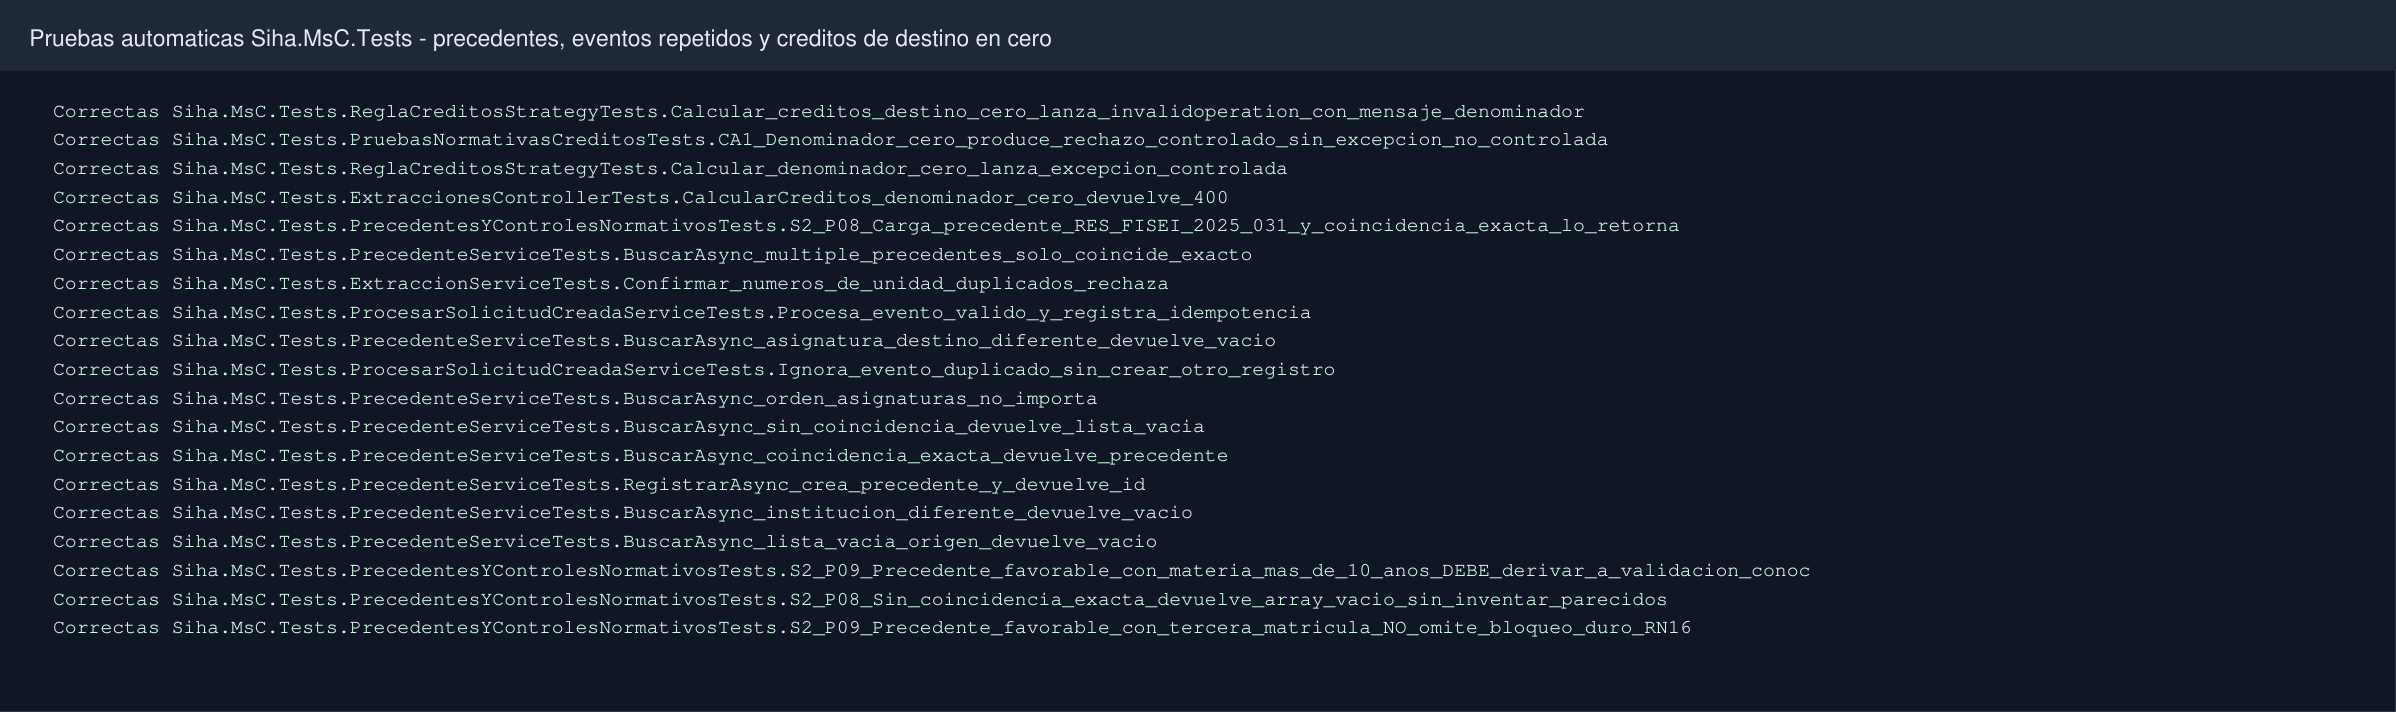
\includegraphics[width=\textwidth]{pa11-automaticas.png}
\caption{Pruebas automáticas de precedentes, avisos repetidos y créditos de destino en cero (HU-09 y HU-11)}
\label{fig:automaticas}
\end{figure}

\begin{table}[H]\centering\small
\begin{tabularx}{\textwidth}{|l|X|X|l|}\hline
\rowcolor{grisTarjeta}\textbf{N.º} & \textbf{Prueba} & \textbf{Resultado obtenido} & \textbf{Estado}\\\hline
PA-07.1 & Lectura de un PDF con texto & Datos completos del certificado & Cumple\\\hline
PA-07.2 & Aviso repetido & Aviso con enlace; un solo análisis & Cumple\\\hline
PA-07.3 & Datos que faltan & ``Campos sin llenar''; no se analiza & Cumple\\\hline
PA-07.4 & Confirmar con datos vacíos & Lista de faltantes; no se guarda & Cumple\\\hline
PA-07.5 & PDF escaneado & ``No es el certificado SIHA'' & Cumple\\\hline
PA-08.1 & Reglas en el resultado & Reglas explicadas por materia & Cumple\\\hline
PA-08.2 & Cambio de umbral & 85~\%, versión 5 (luego 80~\%) & Cumple\\\hline
PA-08.3 & Servicio apagado & ``Se está preparando'' y reintento & Cumple\\\hline
PA-09.1 & Créditos suficientes & 100~\% & Cumple\\\hline
PA-09.2 & Créditos insuficientes & 66,67~\%: no se puede homologar & Cumple\\\hline
PA-09.3 & Destino sin créditos & Rechazo controlado & Cumple (automática)\\\hline
PA-09.4 & Más de 10 años & Rechazado & Cumple\\\hline
PA-09.5 & Tercera matrícula & Regla explicada; bloqueo automático & Cumple\\\hline
PA-10.1 & Escaneado legible & Ya no se reciben escaneados & Reemplazada (C-01)\\\hline
PA-10.2 & Cobertura por unidades & Tabla tema por tema & Cumple\\\hline
PA-10.3 & Parecido bajo el umbral & Unidad no cubierta & Cumple\\\hline
PA-10.4 & Dos materias para un destino & Temas sumados & Cumple\\\hline
PA-10.5 & Misma materia en dos destinos & Rechazado & Cumple\\\hline
PA-11.1 & Coincidencia exacta & \texttt{BuscarAsync\_coincidencia\_exacta\dots} & Cumple (automática)\\\hline
PA-11.2 & Sin coincidencia & \texttt{BuscarAsync\_sin\_coincidencia\dots} & Cumple (automática)\\\hline
PA-11.3 & Caso solo parecido & \texttt{\dots solo\_coincide\_exacto} & Cumple (automática)\\\hline
PA-11.4 & Precedente y más de 10 años & \texttt{S2\_P09\_Precedente\_favorable\dots} & Cumple (automática)\\\hline
PA-11.5 & Falla la búsqueda & Cubierta por el reintento automático (PA-08.3) & Cumple (corregida C-03)\\\hline
\end{tabularx}
\caption{Resultados de las pruebas del Sprint 2 (nueva ejecución)}
\end{table}

% =====================================================================
\clearpage
\subsection{Sprint 3: revisión, decisión y resultado (HU-12 a HU-19)}

\subsubsection{HU-12 -- Registrar con un único certificado SIHA}

\prueba{PA-12.1: Solicitudes registradas}
{El administrador abre Solicitudes.}
{pa12-1-lista-solicitudes.png}{Lista de solicitudes con su estado (HU-12)}
{Cada solicitud muestra el estudiante, el cambio de carrera, las materias pedidas, los docentes revisores y su estado
(Revisión docente, Falta la decisión del administrador o Resuelta).}{0.95}

\prueba{PA-12.2: Revisión previa con lista de verificación}
{El operador sube el certificado E05, que pide homologar una materia reprobada.}
{pa12-2-checklist.png}{Lista de verificación por sección (HU-12)}
{Cada sección del certificado aparece con un visto o una equis y el motivo en lenguaje sencillo; el botón de registrar
queda deshabilitado y explica por qué.}{0.80}

\textbf{PA-12.3: Certificado repetido.} Se comprobó en la PA-07.2: el aviso aparece junto al botón con el enlace a la
solicitud que ya existe.

\subsubsection{HU-13 -- Análisis explicado con los sílabos oficiales}

\prueba{PA-13.1: Análisis materia por materia}
{Se abre la solicitud V05 recién registrada.}
{pa13-1-analisis.png}{Resumen y análisis explicado (HU-13)}
{El resumen indica cuántas materias cumplen y cuántas no se pueden homologar por créditos; cada materia trae su
recomendación, el historial y las reglas del instructivo.}{0.62}

\prueba{PA-13.2: Reintento automático}
{Tras encender de nuevo Ollama (PA-08.3) se vuelve a abrir la solicitud V07.}
{pa13-2-reintento-analizado.png}{La solicitud se analizó sola al volver el servicio (HU-13)}
{La solicitud pasó de ``El agente se está preparando'' a analizada, sin intervención del operador.}{0.95}

\subsubsection{HU-14 -- Movilidad externa}

\prueba{PA-14.1: Solicitud de otra universidad}
{Se abre la solicitud de movilidad externa de la ESPOCH (V06).}
{pa14-1-movilidad-externa.png}{Movilidad externa con sílabos de otra universidad (HU-14)}
{Las materias con sílabo adjunto se comparan con el de la UTA; las que no tienen sílabo quedan ``Sin sílabo para
comparar · decide el docente'' (criterio docente).}{0.95}

\subsubsection{HU-15 -- Regla: los créditos bloquean, los contenidos recomiendan}

\prueba{PA-15.1: Créditos por debajo del 80~\%}
{Se revisa Algoritmos y Lógica de Programación en la solicitud V05 (créditos 50~\%).}
{pa15-1-bloqueada-creditos.png}{Materia bloqueada por créditos (HU-15)}
{``No se puede homologar'' y ``Los créditos no llegan al 80~\%'': no hay botones de voto.}{0.95}

\prueba{PA-15.2: Solo contenidos por debajo del 80~\%}
{Se revisa Sistemas Operativos en la solicitud V03 (contenidos 75~\%, créditos 100~\%).}
{pa15-2-recomendacion.png}{Recomendación que los docentes pueden votar (HU-15)}
{``No llega al 80~\% · recomienda no homologar'', pero los docentes sí pueden votarla (ver PA-16.1).}{0.95}

\subsubsection{HU-16 -- Decisión de los docentes y del administrador}

\prueba{PA-16.1: Voto de un docente}
{La docente María Vaca decide las cuatro materias de V03 y rechaza Sistemas Operativos.}
{pa16-1-voto-docente.png}{Voto de una docente (HU-16)}
{El voto queda guardado con su comentario y la solicitud pasa a ``Revisión docente 1/2''.}{0.95}

\prueba{PA-16.2: Los docentes no coinciden}
{El docente Carlos Paredes aprueba Sistemas Operativos.}
{pa16-2-sin-acuerdo.png}{Docentes sin acuerdo (HU-16)}
{La solicitud pasa a ``Falta la decisión del administrador'' y los docentes ven el aviso del desacuerdo.}{0.95}

\prueba{PA-16.3: Decisión final del administrador}
{El administrador elige No homologar y escribe el motivo. Sin motivo el botón Guardar decisión final queda deshabilitado.}
{pa16-3-decision-admin-formulario.png}{Formulario de la decisión final (HU-16)}
{Solo aparece para la materia sin acuerdo y exige el motivo.}{0.95}

\prueba{PA-16.3 (continuación): Solicitud resuelta}
{El administrador guarda la decisión.}
{pa16-3-decision-admin.png}{Decisión final guardada (HU-16)}
{Sistemas Operativos queda No homologada con la decisión y el motivo del administrador; la solicitud pasa a Resuelta.}{0.95}

\prueba{PA-16.4: Cambiar el voto después de la decisión final}
{La docente María Vaca vuelve a la solicitud e intenta enviar otro voto directamente al servidor.}
{pa16-4-votos-cerrados.png}{Votos cerrados después de la decisión final (HU-16)}
{La pantalla ya no ofrece votar (``El administrador ya dio la decisión final'') y el servidor responde \textbf{409} con
``El administrador ya dio la decisión final de esta solicitud; los votos ya no se pueden cambiar.''}{0.95}

\subsubsection{HU-17 -- Tabla de resultados de la homologación}

\prueba{PA-17.1: Tabla RESULTADO\_HOMOLOGACION}
{Se consulta la tabla en la base del Microservicio C.}
{pa17-1-resultado-homologacion.png}{Resultado por materia en la base de datos (HU-17)}
{Una fila por materia con los porcentajes de contenidos y créditos, la estimación del agente, los votos y el resultado
final; coincide con lo que se ve en la aplicación (por ejemplo, Álgebra Lineal 100~\% / 66,67~\% NO\_HOMOLOGADA y
Sistemas Operativos 1--1 NO\_HOMOLOGADA por decisión del administrador).}{1.0}

\subsubsection{HU-18 -- Registro manual sin PDF}

\prueba{PA-18.1: Llenado automático desde la malla}
{El operador elige Ingeniería Industrial a Software, pulsa Cargar materias de la malla hasta el nivel 2 y elige el período de la primera materia de cada nivel.}
{pa18-1-carga-automatica.png}{Historial cargado desde la malla de origen (HU-18)}
{Se cargan solas las 12 materias de los niveles 1 y 2. El nivel y la materia se eligen de listas, y el período se elige de los períodos de la UTA ya precargados: al elegirlo en una materia se copia a las demás del mismo nivel. Solo falta escribir la nota.}{0.95}

\prueba{PA-18.2: Materias que no se relacionan}
{El operador pide homologar Química por Algoritmos y Lógica de Programación.}
{pa18-2-no-relacionadas.png}{Aviso de materias que no se relacionan y sugerencias (HU-18)}
{Aparece ``Estas materias no se relacionan: «Quimica» no se relaciona con «Algoritmos y logica de programacion» (sus
temas se parecen solo un 2~\%)'' y se ofrecen sugerencias automáticas con materias parecidas.}{0.95}

\subsubsection{HU-19 -- Cuentas y sesión}

\prueba{PA-19.1: Restablecer contraseña}
{El administrador pulsa Restablecer contraseña en la cuenta del operador.}
{pa19-1-restablecer.png}{Restablecer la contraseña de una cuenta (HU-19)}
{Se abre la ventana con nueva contraseña, confirmación y el botón Mostrar; solo el Administrador la ve.}{0.95}

\textbf{PA-19.2: Volver a una página permitida al iniciar sesión.} Lo comprueban las pruebas automáticas de
\texttt{navegacion.test.ts} y \texttt{LoginPage}: después de iniciar sesión solo se vuelve a la página anterior si el
rol la puede ver.

\begin{table}[H]\centering\small
\begin{tabularx}{\textwidth}{|l|X|X|l|}\hline
\rowcolor{grisTarjeta}\textbf{N.º} & \textbf{Prueba} & \textbf{Resultado obtenido} & \textbf{Estado}\\\hline
PA-12.1 & Solicitudes registradas & Lista con estados & Cumple\\\hline
PA-12.2 & Revisión previa & Lista de verificación por sección & Cumple\\\hline
PA-12.3 & Certificado repetido & Aviso con enlace & Cumple\\\hline
PA-13.1 & Análisis explicado & Resumen y explicación por materia & Cumple\\\hline
PA-13.2 & Reintento automático & Se analizó sola & Cumple\\\hline
PA-14.1 & Movilidad externa & Sílabo externo y criterio docente & Cumple\\\hline
PA-15.1 & Créditos bajo 80~\% & Bloqueada, sin voto & Cumple\\\hline
PA-15.2 & Solo contenidos bajo 80~\% & Recomendación votable & Cumple\\\hline
PA-16.1 & Voto de un docente & Revisión 1/2 & Cumple\\\hline
PA-16.2 & Sin acuerdo & Falta la decisión del administrador & Cumple\\\hline
PA-16.3 & Decisión final & Con motivo; solicitud Resuelta & Cumple\\\hline
PA-16.4 & Votos cerrados & Pantalla sin voto y 409 & Cumple\\\hline
PA-17.1 & Tabla de resultados & Filas coherentes con la app & Cumple\\\hline
PA-18.1 & Llenado automático & 12 materias y períodos precargados & Cumple\\\hline
PA-18.2 & Materias no relacionadas & Rechazo y sugerencias & Cumple\\\hline
PA-19.1 & Restablecer contraseña & Ventana solo para Administrador & Cumple\\\hline
PA-19.2 & Página permitida al entrar & Pruebas de navegación & Cumple (automática)\\\hline
\end{tabularx}
\caption{Resultados de las pruebas del Sprint 3}
\end{table}

% =====================================================================
\subsection{Hallazgos de la ronda de pruebas}

\begin{table}[H]\centering\small
\begin{tabularx}{\textwidth}{|l|l|X|l|}\hline
\rowcolor{grisTarjeta}\textbf{ID} & \textbf{Gravedad} & \textbf{Descripción} & \textbf{Estado}\\\hline
H-01 & Baja & El resumen decía ``recomienda no homologar'' para materias bloqueadas por créditos. & Corregido\\\hline
H-02 & Media & La regla RN-01 del catálogo todavía decía que los docentes podían homologar aunque no se llegue. & Corregido (RN-01 2.2)\\\hline
H-03 & Media & En el registro manual, ``Agregar todas las sugerencias'' crea las solicitudes pero deja vacía la materia de destino (diferencia de mayúsculas entre la sugerencia y la lista). & Corregido\\\hline
H-04 & Baja & La página ``Reglas de homologación'' (explicación sencilla) ya no está en el menú ni en las rutas. & Pendiente (decisión del equipo)\\\hline
H-05 & Baja & En el Microservicio B el expediente queda en PENDIENTE\_CONTENIDOS aunque en el C ya esté resuelto. & Pendiente\\\hline
H-06 & Baja & El catálogo muestra los nombres de las materias sin tildes (por ejemplo ``Quimica'', ``Fisica basica''). & Pendiente\\\hline
\end{tabularx}
\caption{Hallazgos encontrados al ejecutar las pruebas}
\end{table}

\begin{figure}[H]\centering
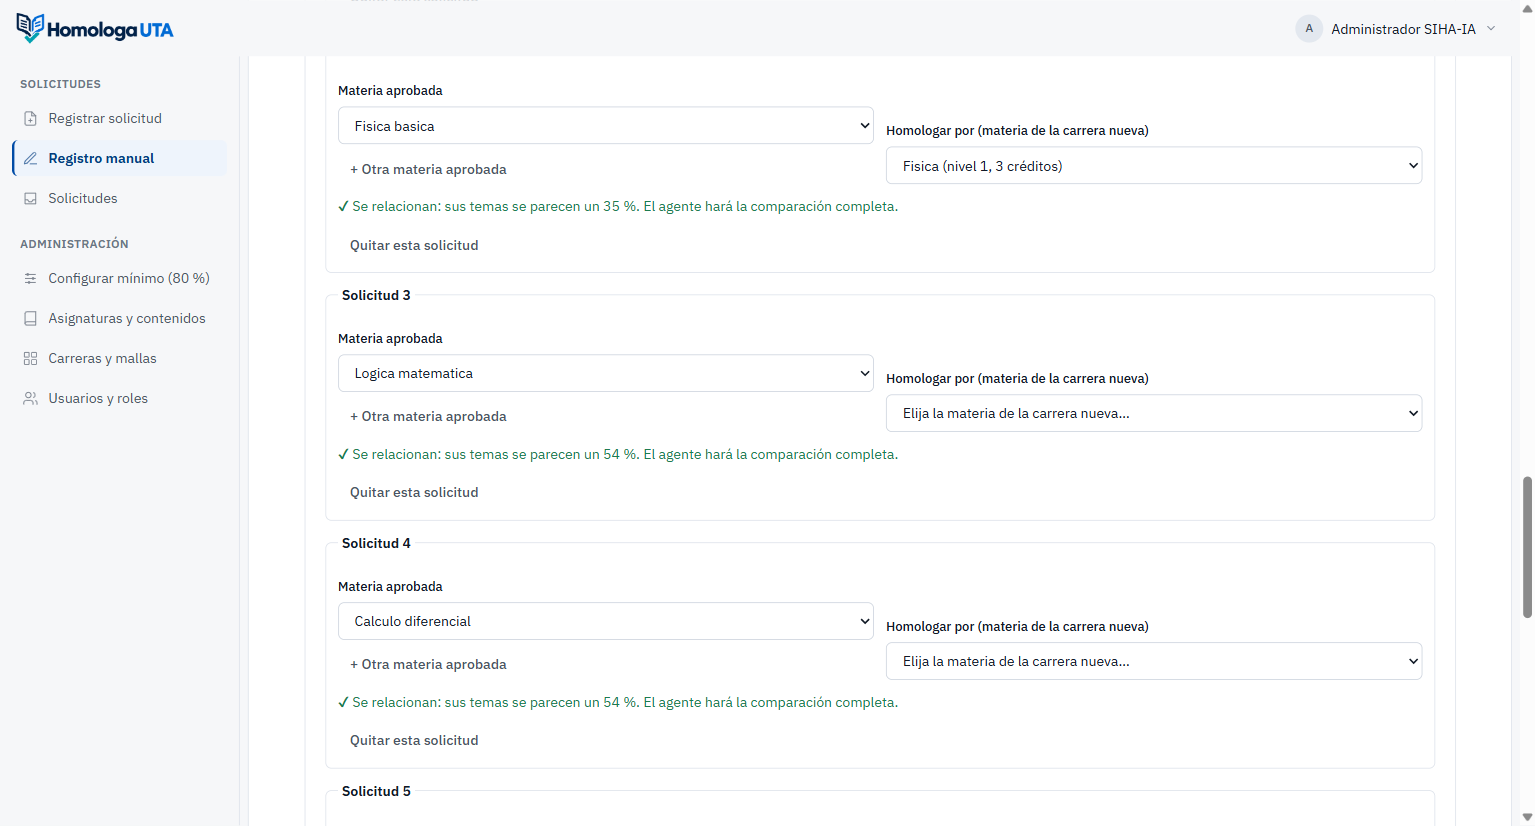
\includegraphics[width=0.85\textwidth]{h-sugerencias-destino-vacio.png}
\caption{Hallazgo H-03 antes de corregirlo: solicitudes sugeridas con la materia de destino vacía}
\end{figure}

La causa de H-03 era que la sugerencia trae el nombre de la materia con otras mayúsculas o sin tildes, y la lista no lo reconocía. Se corrigió para que se elija la materia de la malla que tiene el mismo nombre, y se agregó una prueba automática que lo comprueba.

\begin{figure}[H]\centering
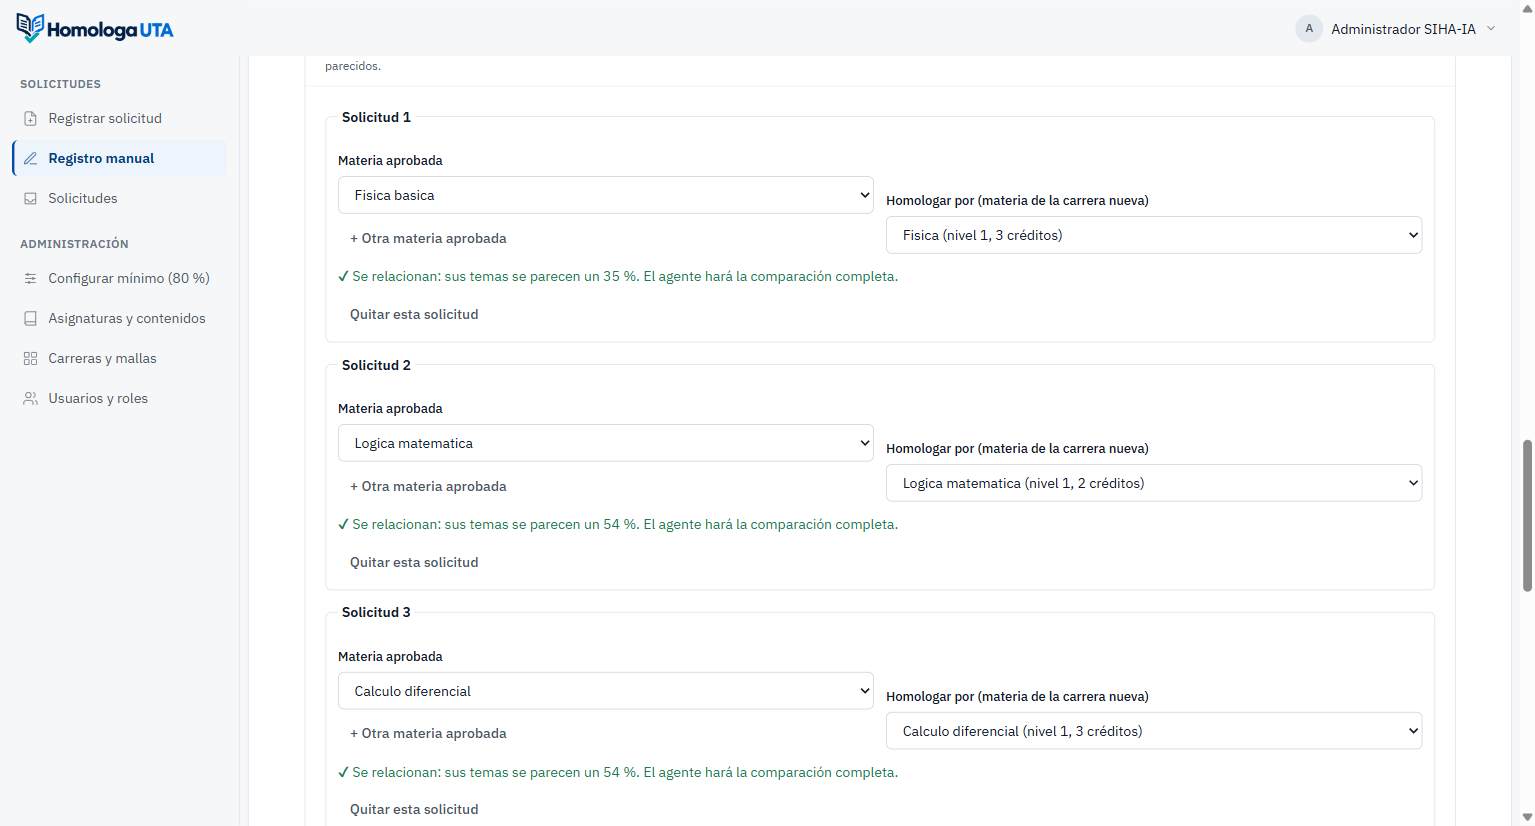
\includegraphics[width=0.85\textwidth]{h-sugerencias-destino-corregido.png}
\caption{Hallazgo H-03 corregido: cada solicitud sugerida ya tiene su materia de destino}
\end{figure}

% =====================================================================
\subsection{Pruebas automáticas}

\begin{table}[H]\centering\small
\begin{tabular}{|l|l|r|l|}\hline
\rowcolor{grisTarjeta}\textbf{Proyecto} & \textbf{Herramienta} & \textbf{Pruebas} & \textbf{Resultado}\\\hline
Microservicio A (usuarios, reglas, catálogo) & xUnit & 130 & Todas correctas\\\hline
Microservicio B (expedientes y certificado) & xUnit & 158 & Todas correctas\\\hline
Microservicio C (agente y decisión) & xUnit & 257 & Todas correctas\\\hline
Interfaz web & Vitest & 99 & Todas correctas\\\hline
Gateway (rutas y permisos) & Node & 26 & Todas correctas\\\hline
\end{tabular}
\caption{Pruebas automáticas al cierre del Sprint 3}
\end{table}

\subsection{Resumen general}

\begin{table}[H]\centering\small
\begin{tabular}{|l|c|c|c|c|}\hline
\rowcolor{grisTarjeta}\textbf{Estado} & \textbf{Sprint 1} & \textbf{Sprint 2} & \textbf{Sprint 3} & \textbf{Total}\\\hline
Cumple & 12 & 16 & 16 & 44\\\hline
Cumple (automática) & 0 & 5 & 1 & 6\\\hline
Cumple (corregida) & 0 & 1 & 0 & 1\\\hline
Reemplazada por una corrección & 0 & 1 & 0 & 1\\\hline
Pendiente & 0 & 0 & 0 & 0\\\hline
\textbf{Total} & \textbf{12} & \textbf{23} & \textbf{17} & \textbf{52}\\\hline
\end{tabular}
\caption{Resumen de los resultados de las pruebas de los tres sprints}
\end{table}

Todas las capturas originales están en la carpeta \texttt{capturas}, nombradas por prueba y en el mismo orden de esta sección.
